%% Briefings in Bioinformatics submission build.
%%
%% WHY THIS FILE EXISTS SEPARATELY FROM ../main.tex. ../main.tex is the internal, venue-agnostic
%% manuscript: no length constraint, Nature-shaped (Results before Methods), and it is where the
%% evidence is worked out. This file is the same evidence in the shape Briefings in Bioinformatics
%% actually publishes, which J8 established is a DIFFERENT shape -- Methods before Results, a ~200
%% word abstract, a Key Points box. Keeping both means the venue-shaped cut can be redone if the
%% venue changes, without having destroyed the long form. Every number here is the same number;
%% `paper/check_numbers.py` reads both.
%%
%% Venue evidence: briefings_in_bioinformatics_lock.json -> j8_completion_20260817, which records
%% what was OBSERVED from three papers BiB published (bbaf103, bbaf521, bbaf121) and what the
%% journal never states. Read it before changing structure here.
%%
%% Class: oup-authoring-template, OUP's own, shipped with TeX Live 2025 -- no download.
%%   /usr/local/texlive/2025/texmf-dist/tex/latex/oup-authoring-template/
%% OUP's manual says the layout options are cosmetic: "you are not responsible for any final page
%% layout ... similar but not identical to the layout of the final article." So contemporary/large
%% is not load-bearing and should not be argued about.
%%
%% Figures are NOT copied here. \graphicspath points at the directory they are built in, because a
%% document reading a copy is unchecked by construction and goes stale silently.

\documentclass[unnumsec,webpdf,contemporary,large]{oup-authoring-template}

\graphicspath{{../figures/}}

\usepackage{afterpage}
\usepackage{booktabs}
\usepackage{siunitx}
\usepackage{xcolor}


%% Placeholders that RENDER LOUDLY. A placeholder whose failure mode is silence -- TBD_GITHUB_URL,
%% an empty field -- ships. One that prints in red does not.
\newcommand{\TODOauthor}{\textcolor{red}{[TODO: author-supplied -- ask, do not infer]}}
\newcommand{\TODO}[1]{\textcolor{red}{[TODO: #1]}}
\newcommand{\TODOport}[1]{\textcolor{red}{[TODO: #1]}}

\journaltitle{Briefings in Bioinformatics}
\DOI{}
\copyrightyear{2026}
\pubyear{2026}
\access{}
\appnotes{Problem Solving Protocol}

\firstpage{1}

\begin{document}

%% Title, third version. The first ran to 43 words. The second said "a corrected clinical
%% baseline", which frames a primary paper as an erratum, and the word is wrong anyway: the finding
%% is WHICH VARIABLE is absent, not that a baseline was repaired. Every compact way of putting the
%% finding IN a title fails one of two ways -- "corrected baseline" reads as housekeeping, and
%% "stage-aware" claims as an innovation what is simply the honest specification of a clinical
%% block. So the title lists the three inputs instead, and pathologic stage appears among them
%% without being claimed. A reader who knows this benchmark will notice it is there; the abstract
%% says why that is worth noticing.
\title[Parameter-free multimodal fusion in bladder cancer survival]{ModRank: parameter-free fusion
of histology, transcriptome and pathologic stage for bladder cancer survival}

%% Author identity supplied by the author 2026-08-17. ORCID from the same record.
\author[1,$\ast$]{Guanxing Chen\ORCID{0000-0002-4435-0884}}
\authormark{Chen}
\address[1]{\orgname{City University of Hong Kong (Dongguan)}, \orgaddress{\street{Dongguan}, \country{China}}}
\corresp[$\ast$]{Corresponding author. \href{mailto:guanxing.chen@cityu-dg.edu.cn}{guanxing.chen@cityu-dg.edu.cn}}

\received{}{0}{}
\revised{}{0}{}
\accepted{}{0}{}

\abstract{After cystectomy, pathologic stage is the strongest routine predictor of how muscle-invasive
bladder cancer will behave, and it does not say which patients within a stage will die of it. Progress on closing it is measured almost entirely on one benchmark, the five-fold splits of TCGA disease-specific survival released with SurvPath. We read the method papers on its bladder cohort, eight of the eleven in full. Four report a clinical-variable baseline and \textbf{every one builds it from tumour grade}. \textbf{Not one uses
pathologic stage}, and four more report no clinical baseline at all. Grade cannot separate these patients: two levels, 94.4\% in one, entropy 0.311. Stage is not
missing. It ships with the benchmark, in the same files. Rebuilt from them it reaches 0.6638 against 0.5666 for the grade construction on identical cases (95\% CI $[+0.047,\,+0.149]$, $p<0.001$), and beats the incumbent clinical arm in all five TCGA studies the benchmark covers. Measurement then dictates the method: at 359 patients and 113 events a ridge Cox fitted to pure noise scores 0.7474 in-sample. ModRank
therefore fits one penalised Cox model per modality and averages their ranks with equal weights,
fitting nothing in the combination. Under a protocol frozen before the run it reaches 0.7212 with 1,049 parameters against two competitors' 25 million. The rule's own selection correction was mis-specified and we report that: measured against a permuted-outcome null it does not clear the corrected bar. That is \textbf{state of the art by the convention this benchmark is ranked on}, a comparison of point estimates we show cannot resolve the ordering it is used for.}

\keywords{computational pathology; survival analysis; bladder cancer; benchmarking; multimodal
integration; clinical baselines}

%% KEY POINTS. BiB requires 3-5 brief sentences (observed: 4/3/3 bullets across the three sampled
%% papers). The journal displays them at the end of the article. The template's own tag for them is
%% front matter and OUP's typesetter does the moving, so \boxedtext here is correct even though the
%% published position is different.
\boxedtext{
\begin{itemize}
\item On the TCGA-BLCA whole-slide survival benchmark, every method paper we could read that
  reports a clinical-variable baseline builds it from tumour grade and none uses pathologic stage,
  and half of the papers we read report no clinical baseline at all. Stage is a column in the released files,
  including the split files of the current best method.
\item The failure is structural and specific to this disease: muscle-invasive urothelial carcinoma
  is 94.4\% one grade level, so the covariate the field has been comparing against cannot separate
  the patients it does not distinguish.
\item Rebuilt with stage, the clinical baseline reaches 0.6638 against 0.5666 for the grade
  construction, and it exceeds two of the four published entries on verified folds and five of
  all nine the benchmark carries.
\item \textbf{ModRank}, a method chosen by measurement rather than architecture (one penalised Cox per modality, combined by an equal-weight rank average with no fitted parameter), reaches 0.7212 with 1,049 parameters against competitors carrying 25 million, the highest value reported on these folds by the point-estimate convention every entry is ranked by. Its own pre-registered selection correction was mis-specified, and against a permuted-outcome null the value does not clear the corrected bar. We report both.
\end{itemize}}

\maketitle

\section{Introduction}
Bladder cancer is the tenth most common cancer worldwide, with more than 600,000 new cases a year
and roughly 220,000 deaths~\citep{bray2024globocan}. About a quarter of patients present with
muscle-invasive disease. For those treated by radical cystectomy, the pathologic stage of the
specimen is the strongest routine predictor of what happens after surgery, and it guides what
follows it: whether adjuvant treatment is considered and how closely the patient is
followed~\citep{witjes2021eau}. Stage is also, by construction, a
coarse instrument. Two patients with pT3 N0 M0 disease receive the same recommendation and do not
have the same outcome, and the report holds nothing that separates them. That residual
heterogeneity is real and it is molecular: a consensus classification places muscle-invasive
tumours into six transcriptomic classes with markedly different survival, and those classes cut
across stage~\citep{kamoun2020consensus, tcga2014blca}. The clinical question this paper is
positioned against is therefore not whether stage predicts outcome. It is what can be added to
stage.

Computational pathology answers that question with the slide itself. A whole-slide image carries
morphology no staging category encodes, and weakly supervised aggregation over its tiles made
slide-level prediction practical without region
annotation~\citep{lu2021clam, chen2024uni, ding2025titan}. Bulk transcriptomics carries
programme-level state that morphology does not, and the multimodal premise is that a model reading
both can order patients whom stage orders identically. Progress toward that premise is measured, in
practice, on one benchmark. SurvPath released five-fold case-identifier splits for TCGA
disease-specific survival across five studies~\citep{jaume2024survpath}, and its bladder cohort of
359 cases and 113 events has since carried at least eleven method papers, from
MCAT~\citep{chen2021mcat} and MOTCat~\citep{xu2023motcat} through MMP~\citep{song2024mmp},
PIBD~\citep{zhang2024pibd}, OTSurv~\citep{ren2025otsurv}, DSCASurv~\citep{song2025dscasurv} and
DIMAF~\citep{eijpe2025dimaf}. Reported concordance on it has moved from 0.596 to 0.679.

On this benchmark the clinical baseline is either specified without stage or absent altogether
(Fig.~\ref{fig:overview}a). The census is Supplementary Table~S1. Eight of the eleven papers
could be read in full: four report a clinical-variable baseline, all four build it from tumour
grade, and not one of the eight uses pathologic stage. The other three are marked unverified
rather than assumed to follow the pattern. The bladder values reported are 0.519 (DIMAF) and 0.570 (MMP, and the same figure in
SurvPath's own table), and SurvPath's age-alone arm reaches 0.578 (MMP). A concordance of 0.519 for
the clinical arm, in a disease whose staging guides post-operative care, is a claim that the routine
pathology report is a coin flip. The variable that would have avoided it ships with the benchmark:
the released clinical table carries stage, grade and subtype for all five studies, and DIMAF's own
split files carry the AJCC pathologic tumour stage directly beside the histological grade. The
mechanism behind the choice is specific to this disease and is the reason it went unnoticed.
Muscle-invasive urothelial carcinoma is almost uniformly high grade. In this cohort grade
takes two levels with 94.4\% of cases in one of them and normalised Shannon entropy
0.311 (Fig.~\ref{fig:overview}d), against five levels and 0.665 for stage. A covariate
that does not distinguish the patients cannot separate them, whatever model is fitted on top of it.

That a clinical reference should be strong is not a new idea, and saying so is what turns this
from a complaint into a finding. The multi-omics survival literature has argued for years that
molecular blocks add little over clinical covariates on TCGA, and it has argued so \emph{with the
right covariates}. Herrmann and colleagues benchmarked survival methods across 18 TCGA cohorts,
bladder among them, against a Cox reference using ``sex, age, histological type and tumor
stage''~\citep{herrmann2021benchmark}, in this journal, in 2021. Wissel and colleagues reached the
same conclusion on 17 TCGA datasets against a clinical set that likewise included ``tumor stage,
clinical stage''~\citep{wissel2023noise}. Neither used whole-slide images, and that is the whole of
the gap. The whole-slide survival family is a separate literature published at vision and
medical-imaging venues, and it did not inherit the correction: its own earlier work set the
pattern, with PORPOISE comparing against ``Cox proportional hazard models using age, gender, and
tumor grade covariates'' across fourteen cancer types~\citep{chen2022porpoise}. Our contribution
is therefore not the observation that a clinical baseline is strong. It is that one identifiable
body of work has been measuring the value of morphology against a covariate its own neighbours had
already discarded, that the failure is mechanical rather than careless, and that correcting it
reorders the published table.

The second observation is about the regime rather than the field, and it decides what a method
should look like here. Three hundred and fifty-nine patients and 113 events is a small survival
problem, and small survival problems punish parameters: the events-per-parameter arithmetic behind
modern sample-size guidance rules out fitting a large fusion network on a cohort this
size~\citep{riley2020samplesize}. We measured what that costs before designing anything. A ridge
Cox fitted to pure noise and scored in-sample reaches 0.7474 at sixteen parameters, an oracle
fusion whose two weights are fitted on the held-out fold is worth only $+0.008$ over equal
weighting, and a gated combination loses to its own permuted-stratum control. The three answers
point the same way. On this benchmark the binding constraint is estimation, so a method should
spend its events on the coefficient vectors that carry signal and none on the combination.
ModRank does exactly that and nothing more: one penalised Cox model per modality over
frozen representations, percentile normalisation within fold, and an equal-weight rank average with
no fitted parameter in the combination. It carries 1,049 coefficients in total, and it reaches the
highest concordance reported on these folds.

\begin{figure*}[t]
\centering
\includegraphics[width=\textwidth]{fig1_overview.pdf}
\caption{\textbf{The defect, the method, and the protocol.}
\textbf{(a)} The files released with the benchmark carry histological grade and AJCC pathologic
tumour stage one row apart. Every method paper that reports a clinical
baseline at all builds it from the first. The second reaches 0.6638 against 0.5666 on identical cases
through an identical pipeline.
\textbf{(b)} The method: one penalised Cox per modality over a frozen slide embedding,
pathway-level transcriptomics and the staging variables, combined by an equal-weight rank average
with no fitted parameter in the combination. 1,049 coefficients in total, against 24.7 and 26.9
million for the two competitors whose code we could rerun.
\textbf{(c)} The protocol, and what was fixed before the number existed.
\textbf{(d)} Why grade cannot work here: it takes two levels with 94.4\% of cases in one of them,
normalised entropy 0.311, against five levels and 0.665 for stage.}
\label{fig:overview}
\end{figure*}


\section{Materials and methods}
%% METHODS BEFORE RESULTS. Observed in 3 of 3 sampled BiB papers. This is the largest structural
%% difference from ../main.tex and it is not a preference.
\subsection{Cohort and endpoint}

TCGA-BLCA, disease-specific survival, as defined by the metadata SurvPath
releases~\citep{jaume2024survpath}: its disease-specific survival time and censoring
indicator, which derive from the
TCGA Pan-Cancer Clinical Data Resource~\citep{liu2018tcgacdr}. A case has an event when
the censoring indicator is zero.

The prediction this benchmark scores is a post-operative one. The tumours had not been exposed
to chemotherapy when the tissue was acquired~\citep{robertson2017blca}, the stage is the
pathologic stage of the resected specimen, and survival runs from the date of initial pathologic
diagnosis, the origin the resource uses for every endpoint~\citep{liu2018tcgacdr}. A score of this
kind can inform adjuvant treatment and follow-up. It cannot inform the decision to give
neoadjuvant chemotherapy, which is taken before the specimen exists.

The analysis cohort is the intersection of cases holding a slide embedding and a disease-specific
survival label: 359 cases, 113 events, 24{,}219 comparable pairs. That is exactly the set
the released folds partition, so no case is dropped by our pipeline that the benchmark includes.
A case may hold several slides. Slide-level features are mean-pooled to the case before anything
else, and a case is the unit throughout.

\subsection{Splits}

The five fold files SurvPath released for bladder, used verbatim and never regenerated.
Fold sizes (train/validation, cases): 289/70, 287/72, 284/75, 288/71, 288/71. We obtained them from
the PIBD repository~\citep{zhang2024pibd} and confirmed byte by byte that all five files are
byte-identical to SurvPath's.

A canonical membership manifest (per fold, the fold index and the comma-joined sorted train and validation case identifiers, newline-joined) is recorded in
a machine-readable split manifest whose SHA-256 is bound into the frozen protocol so that a
later run cannot silently use a different partition.

\paragraph{Verifying the comparators' folds.} Fold identity is the axis on which these results are
or are not comparable, and it is not uniform across the field, so we checked it rather than assuming
it. PIBD ships the released files unchanged. DIMAF~\citep{eijpe2025dimaf} ships
its own five-fold split files at \emph{slide}
granularity. Collapsing them to the case identifier reproduces the released partition exactly: five of five validation folds identical, the 359-case universe identical, and no case in one but
not the other.

The rest cannot be checked. APL's repository contains two files. MMP states its own site-stratified
protocol and OTSurv follows MMP, so neither uses the released partition. MOAD-FNet and DSCASurv
release no split files at all. Values from that group are listed separately wherever they
appear, and are excluded from the comparison the paper's claim rests on.

\subsection{Representations}

\paragraph{Morphology.} A 768-dimensional TITAN slide embedding~\citep{ding2025titan} per whole-slide
image, taken from a public precomputed release covering 11{,}658 TCGA diagnostic slides, mean-pooled
over a case's slides. No slide-level model is trained here.

\emph{On the encoder's provenance}, because a frozen embedding is the one place a linear model could
inherit information it did not earn: TITAN was pretrained on 335{,}645 whole-slide images collected
internally at Mass General Brigham, by visual self-supervised learning and vision-language alignment
against pathology reports and synthetic captions. No patient outcome or survival label
enters its pretraining, and its authors state that it did not use TCGA, PAIP, CPTAC or PANDA, the
public collections benchmarks are built from. So the embedding cannot have seen this cohort's
slides, and could not have seen its endpoint even if it had. The within-site column of
Table~\ref{tab:main} is the residual check on the weaker version of the same worry, that a
site-level signature correlated with outcome survives pooling.

\begin{table*}[t]
\centering
\caption{Confirmatory result and its comparators, \textbf{all at seed 0}, the protocol's reference
seed. All arms use the same folds, the same estimator and the same clinical block. ``tied''
restricts the concordance to the decile of comparable pairs the clinical arm separates least. The
primary metric below is the mean over seeds 0--4 and the paired comparisons reported later use
seed-averaged scores. The three quantities are distinguished in the text because they are not
interchangeable.}
\label{tab:main}
\begin{tabular}{lccc}
\toprule
arm & C-index & tied (q10) & within-site \\
\midrule
clinical, age+sex+grade   & 0.5666 & 0.4800 & 0.5535 \\
clinical, age+sex+stage   & 0.6638 & 0.5107 & 0.6561 \\
omics (275 pathways)               & 0.6510 & 0.6422 & 0.6533 \\
slide embedding                    & 0.6596 & 0.6271 & 0.6334 \\
SurvPath, official rerun           & 0.6118 & 0.5999 & 0.6028 \\
SurvPath + the same clinical       & 0.6810 & 0.6040 & 0.6708 \\
ours, slide + omics only           & 0.6841 & 0.6581 & 0.6618 \\
ours                      & \textbf{0.7225} & \textbf{0.6634} & \textbf{0.7093} \\
\bottomrule
\end{tabular}
\end{table*}

\paragraph{Transcriptome.} SurvPath's own 4{,}999-gene matrix for bladder, averaged into the 275 pathway groups its own
signature definitions specify that carry at least three of those genes.
This is close to what SurvPath's omics branch itself consumes, and using the benchmark's own
grouping avoids a representation chosen by us in a place where a choice would be hard to justify.

\paragraph{Clinical.} Age, sex and pathologic stage, one-hot for the categorical, taken from
\emph{DIMAF's own released split files}: age at diagnosis, sex and
AJCC pathologic tumour stage. The grade contrast uses the histological grade field from
the same files. Taking the clinical block from the incumbent's own repository removes any question
of whether ModRank sees information the comparators did not.

Three cases carry an incomplete record and are handled without being dropped, because dropping them
would change the cohort the comparison is made on. One case has no birth date and is given the
cohort's rounded median age of 65 years. Two cases carry no stage and two carry no grade. A level
recorded as unavailable, unknown or not evaluated produces an all-zero indicator row rather than a
level of its own, so those cases sit at the encoding's reference point and contribute no stage or
grade information. All 359 cases are scored.

\paragraph{Representations that were evaluated and not used.} Six further public precomputed
slide-level feature releases were scored as additional views: the native Prov-GigaPath slide
encoder~\citep{xu2024provgigapath} at all fourteen layers, four GigaSSL aggregations (over Phikon,
H-Optimus-0, Prov-GigaPath and CTransPath~\citep{wang2022ctranspath} tile features), and mean-pooled
UNI~\citep{chen2024uni} patch features. None beat TITAN (0.6051, 0.6004, 0.5807, 0.5802, 0.5328 and
0.5224 against 0.6596), their pairwise rank correlations run 0.63--0.69 so they are not independent
views, and an ensemble of all seven is \emph{significantly worse} than TITAN alone ($-0.0440$, 95\%
CI $[-0.0781,-0.0108]$, $p=0.008$). The UNI release carries roughly 21 patches per slide, a far
coarser tiling than the prototype aggregation MMP and DIMAF use, which is the visible reason its
mean pool is weak.

\subsection{Estimator}

One ridge-penalised Cox proportional-hazards model~\citep{cox1972regression,simon2011regularization}
per view, maximising the Breslow-tie partial likelihood by L-BFGS on the exact objective and its
analytic gradient. The penalty $\alpha$ is chosen from $\{1, 8, 64, 512, 4096\}$ by three-fold
inner cross-validation \emph{inside} the training fold, with the concordance of the
out-of-inner-fold predictions as the criterion. Standardisation uses training-fold means and
standard deviations only. The estimator is identical for every view.

\paragraph{Why the estimator is not selected per view.} It could be, and we measured what that
costs. Choosing among $\{$plain ridge, dense-grid ridge, bagged ridge$\}$ per view by inner
cross-validation gives 0.6568, 0.6543 and 0.6743 for the morphology, transcriptome and clinical
views against 0.6596, 0.6510 and 0.6856 for plain ridge everywhere, measured during development
while the clinical view was still the earlier block that Amendment~A1 replaced: selection
\emph{cost} performance on two views of three. At 287 training patients the inner criterion cannot reliably
separate estimators that differ by 0.02, so adaptive selection buys noise at full price.

\subsection{Combination}

Out-of-fold predictions are percentile-normalised to $[0,1]$ \emph{within each fold}, identically
for every arm, and then averaged with equal weights. We call the resulting method ModRank,
for modality-wise rank averaging, and the name is meant to carry the constraint rather than an
architecture: beyond fitting one penalised Cox model per modality, ModRank only puts the three scores on a common rank scale and takes their mean, so the combination has no
parameter to fit and none to overfit. The normalisation is not cosmetic: without it
a Cox log-hazard on one fold's scale is pooled against another's, and the pooled concordance
measures scale rather than skill.

\paragraph{The transform, stated exactly, and the inductive variant of it.} For fold $k$ with
validation set $V_k$, arm $m$'s normalised score for case $i \in V_k$ is
$z^{m}_{i} = \mathrm{rank}\big(s^{m}_{i};\, \{s^{m}_{j}\}_{j \in V_k}\big) / (|V_k| - 1)$, where
$s^{m}$ is the fitted arm's linear predictor. The reference set is the validation fold
itself, which makes the transform transductive: a case's normalised score depends on the other
cases being scored beside it. No outcome enters it, and it cannot change any single arm's
concordance, a within-fold monotone map leaves that arm's own ranking untouched, but it can
move the combination, because the rank average depends on how the three arms are scaled relative to
one another.

So we ran the deployable alternative and report it. In the \emph{inductive} variant the reference
set is the training fold's own predicted scores, $z^{m}_{i} = \hat{F}^{m}_{\text{train}}(s^{m}_{i})$,
which a single new patient could be scored against with nothing else present. It reaches
0.7247 against the transductive 0.7212. The deployable version is if anything slightly
\emph{better} (paired difference $+0.0019$, 95\% CI $[-0.0075,\,+0.0112]$, $p=0.69$). We report the
transductive figure as the primary because it is what the frozen protocol specified, and record
here that nothing rests on the choice.

The equal weighting is a measured choice~\citep{bates1969combination}. A 21-point sweep of
$w\,z_{\text{image}} + (1-w)\,z_{\text{clinical}}$ peaks at exactly $w=0.50$. A two-parameter Cox
fusion \emph{fitted in-sample on the held-out fold} reaches 0.7268 against equal weighting's 0.7191,
so even oracle-fitted weights are worth $+0.008$. A fusion whose image weight is gated on
clinical-risk tertile reaches 0.7493 against a permuted-stratum control at 0.7502. The control
wins, and the pre-registered consequence is that the component is void. No parameter in the
combination is fitted.

\subsection{Evaluation and uncertainty}

Harrell's concordance index~\citep{harrell1982cindex}, pooled over all out-of-fold predictions after
within-fold percentile normalisation. The primary metric is the mean over inner-cross-validation
seeds $0$--$4$, reported with the standard deviation across seeds. Three uncertainties are computed
and they answer different questions:

\begin{enumerate}
  \item Split-reseed floor. The same 359 cases re-split 24 times under an identical
    estimator, alpha grid, inner-CV seed and code path. The paired between-arm delta has
    $\mathrm{SD}=0.0073$. Twice that, $0.0145$, is what a claim must clear to survive a reader
    re-running the study.
  \item Selection inflation. $\sigma\sqrt{2\ln N}$ with $\sigma=0.0073$ and $N=211$, the
    number of candidates the iteration ledger held when the protocol was frozen (that ledger is
    generated from the runs' own output rather than hand-kept). This is $0.0239$, and
    $0.679+0.0239=0.7029$ is the pre-registered target. The campaign finished at 269 candidates,
    all of them scored before the confirmatory run, and the same term over 269 is $0.0244$ for a
    bar of $0.7034$. Both are reported, because the frozen figure is the smaller of the two.
    Both rest on the wrong standard deviation, as the Results show, and neither is used as a test
    the result passes.
  \item Case-level bootstrap. 6{,}000 replicates resampling \emph{cases}, never comparable
    pairs, because pairs sharing a patient are not independent. Where a restricted pair set is used, the ``clinically tied'' decile, the threshold is recomputed inside each replicate, so it
    is a property of the resampled cohort rather than of the original one.
\end{enumerate}

\paragraph{The clinically-tied restriction.} Comparable pairs are ranked by the absolute difference
in the clinical arm's own out-of-fold risk, and the smallest decile (2{,}423 of 24{,}219) is
retained. This isolates pairs of patients whom stage cannot separate, which is the clinically
substantive question and which no paper on this benchmark reports.

\paragraph{The within-site restriction.} Pairs whose two cases share a TCGA tissue source site.
Only 1{,}765 of 24{,}219 pairs qualify, so differences of $\approx0.006$ between arms in that column
are not readable. It is reported as a coarse batch check, not as a comparison.

\subsection{Leakage falsifiers}

Five, executed \emph{before} the protocol was frozen. Two are designed to reject and did.

\begin{itemize}
  \item L1, fold integrity. Train and validation disjoint in all five folds, and all 359 cases sit in
    exactly one validation fold. The fold assignment asserted identical to the one the SurvPath
    rerun used, so the paired comparison is paired. Passed.
  \item L2, no fitting across the boundary. A \emph{mutation} test: refitting the same arm with
    standardisation moments taken from the whole cohort moved the score from 0.6596 to 0.6542. The
    point is that it moved. A test that cannot detect the leak it guards against has not passed.
    Passed.
  \item L3, planted label. A column rebuilt per fold: standard normal on every training row, the
    outcome ordering on every validation row. It moved the score by $-0.0006$. Rejected, as
    designed.
  \item L4, case alignment. Permuting which feature row belongs to which case, outcome held fixed,
    over 30 draws: $0.5127 \pm 0.0369$, within three standard errors of chance.
    Rejected, as designed.
  \item L5, outcome provenance. Zero mismatches between our per-case $(\text{time}, \text{event})$
    and the SurvPath rerun's, so the paired comparison is on one endpoint. Passed.
\end{itemize}

\paragraph{A falsifier that was wrong first.} L3's first version built \emph{one} planted column for
the whole cohort, writing the outcome ordering into each case's row while that case sat in its
validation fold. Because every case is in exactly one validation fold, which L1 had just established, the column ended up encoding the outcome everywhere, including in the four folds
where each case is a training row. The pipeline then learned from real information and scored
0.8715, which the test reported as a leak. It was not one. A planted column that is noise in
training and outcome in validation cannot be a single column. It has to be rebuilt inside each fold,
which is what the version above does.

\subsection{Protocol freeze, and its one amendment}

The frozen protocol fixes the arm, the estimator, the alpha
grid, the combination rule, the comparator set, the seeds and the decision rule, and it was written
after the falsifiers ran and before the confirmatory run. Seeds 1--4 had never been executed at the
time of the freeze. On a benchmark with no held-out split they are the only genuinely unseen axis,
and they were included to catch an arm that works under one inner-cross-validation partition only.
The decision rule as frozen was: primary $> 0.679 + 0.0239$, \emph{and} standard deviation across
seeds $\leq 0.0145$.

\paragraph{Amendment A1.} While verifying DIMAF's fold identity we found a defect in our own
clinical block. It had taken stage and T/N/M from a cached clinical query that selected the
\emph{first} diagnosis record per case. Of the 359 cases, 217 carry more than one diagnosis, and 61 had
their T or stage change once the correct record was chosen. For example, TCGA-SY-A9G0 carries both
``Stage IIB / T2 N0 M0 / Adenocarcinoma, NOS'' and ``Stage IV / T4 N1 M0 / Transitional cell
carcinoma''. The cached file took the first. The tell was present and unread beforehand: Stage IIA,
IIB and IIC appear in that record and are not AJCC bladder stages at all, and the errors were
systematic, understating stage, because the first-listed diagnosis tends to be the earlier or the
other tumour.

The block was rebuilt from DIMAF's own released files, as described above. Two changes landed at once and they pull in opposite directions, so both are given. Fixing the defect alone is worth
$+0.0129$ on the clinical arm and $+0.0050$ on ModRank (95\% CI $[-0.0117,+0.0219]$,
$p=0.56$), so the pre-amendment result was \emph{not} inflated by the defect. But the rebuilt
block takes every clinical column from the incumbent's own files, which \emph{drops} the T, N and M
our cached query had supplied, and that is worth $-0.0110$.

Net, the reported primary fell from 0.7260 to 0.7212, a move of $-0.0048$ and the same size
as the seed-to-seed SD. We report the lower, more conservative arm. Both values exceed the target
as it was frozen, and the Results show why that target was itself mis-specified. The amendment is recorded in the protocol with
all four blocks measured. The conservative arm, every clinical column from the incumbent's own
files, is the one reported, not the higher-scoring variant that adds T, N and M from an external
clinical query under a selection rule of our own design.


\subsection{Software and reproducibility}

Python 3.8.20, NumPy 1.24.4, SciPy 1.10.1, single host, CPU only. The method trains no network and
the confirmatory run takes minutes. The library versions are pinned because the same code on the
same split under a different numerical stack has been shown elsewhere to move a baseline by more
than the margins this area publishes.

\paragraph{Availability.} Everything needed to recompute the numbers reported here is archived under
the identifier given in Code availability. The frozen protocol, the split manifest with its hash,
the iteration ledger covering all 269 scored candidates, the error atlas, the component
pre-registrations with their controls, and the confirmatory run with its logs and environment record
are all included.

\section{Results}
\subsection{The benchmark's clinical baseline omits pathologic stage}

Table~\ref{tab:published-clinical} reproduces the clinical-variable baselines the primary papers
report on the released folds. Supplementary Table~S1 is the census one paper at a time:
which of them report a clinical-variable baseline, what covariates each names verbatim, and which
could not be verified and why. Across every paper that reports
one, and all five studies, the covariates are age, sex and grade. Figure~\ref{fig:missing} is the whole of what follows in one place: where the
corrected baseline sits among the published entries, that the same one-column swap helps in every
study the benchmark covers, and that it helps most where grade is least informative.

\begin{table*}[t]
\centering
\caption{Clinical-variable baselines as published on the released folds, from the primary tables
(SurvPath Supplementary Table~3; MMP Table~1; DIMAF Table~1). No paper we could read in this
benchmark family reports a baseline using pathologic stage or T, N and M.}
\label{tab:published-clinical}
\begin{tabular}{lcccc}
\toprule
cohort & age & sex & grade & age+sex+grade \\
\midrule
BLCA     & 0.578 & 0.489 & 0.515 & 0.570 \\
BRCA     & 0.496 & 0.490 & 0.597 & 0.563 \\
COADREAD & \textbf{0.357} & 0.542 & not reported & 0.655 \\
HNSC     & 0.517 & 0.486 & 0.547 & 0.512 \\
STAD     & 0.499 & 0.529 & 0.552 & 0.592 \\
\bottomrule
\end{tabular}
\end{table*}


We rebuilt the clinical arm twice from the same source, differing in one column. Every covariate
comes from DIMAF's own released split files, so the comparison is
internal to a single pipeline on a single set of cases, and no data enters that the incumbent did
not already hold. On bladder, the grade construction reaches 0.5666 and the stage construction
0.6638: a gap of +0.0972 (95\% CI $[+0.047,\,+0.149]$, $p<0.001$, 6{,}000 replicates
resampling cases, the same instrument every other comparison in this paper uses, and the only
comparison in it that clears significance decisively). Inside ModRank the same swap is worth +0.0369
(0.6856 against 0.7225).

\paragraph{Two clinical sources, and which number comes from which.} The bladder figure above and
the five-study figures below are \emph{not} the same construction, and reading them as one is the
easiest mistake this section invites. The bladder headline takes every clinical column from
DIMAF's own released split files (the incumbent's files, which is what makes it a statement about the incumbent's own baseline) and gives $0.6638$ against $0.5666$, a gap of
$+0.0972$. The five-study comparison takes them from SurvPath's
its own released clinical files instead, because that is the only source that exists for all
five studies, and on bladder the same swap there is worth $+0.0560$ from $0.5658$ to $0.6218$.
Both are real, both are internal to one pipeline on one set of cases, and neither is derived from
the other. Every clinical number in this paper is tagged with its source in
Supplementary Table~S2.

The pattern is not specific to bladder. Repeating the swap on the four other studies the benchmark
covers, using SurvPath's own released clinical files and the same estimator, stage beats grade
in five of five, but only three of those five carry a usable grade column, and in
BRCA and COADREAD the ``grade'' arm is therefore age and sex alone, which is a weaker comparison
and is marked as such wherever it appears: BLCA $+0.0560$, BRCA $+0.0858$, COADREAD $+0.2208$, HNSC $+0.0423$, STAD
$+0.0461$.

\paragraph{A caveat that travels with this result.} Our rebuilt \emph{grade} baseline does not
reproduce the published one, and the gaps are not small: $-0.0042$ on BLCA but $-0.1860$ on
COADREAD. For COADREAD the reason is visible: SurvPath's clinical file carries no usable grade
for that cohort, so our age+sex+grade arm is numerically identical to age+sex, and whatever produced
the published 0.655 is not the construction this file supports. The published values are therefore
\emph{context} for this section, not its comparator. The load-bearing comparison is the internal
one, our grade arm against our stage arm, and it is the only one this claim rests on.

\begin{figure*}[t]
\centering
\includegraphics[width=\textwidth]{fig2_missing_variable.pdf}
\caption{\textbf{The missing variable, quantified.} \textbf{(a)} The nine published entries, ModRank and the two clinical constructions. The dashed rule marks the stage-based clinical arm. Two of the four published entries on
verified folds fall below it, and five of all nine. Entries whose folds could not be verified are
drawn open. \textbf{(b)} The census behind the
claim, one row per paper. Four of the eight papers whose text could be read report a
clinical-variable baseline, all four build it from tumour grade, and none of the eight uses
pathologic stage. The three that could not be read carry a bar rather than an inferred mark.
\textbf{(c)} The same one-column swap in all five studies
the benchmark covers, each on its own cases. \textbf{(d)} The swap buys most where grade is least
informative. Three cohorts carry a usable grade, and the panel says so inside itself because a
correlation printed beside three points reads as an estimate.
\textbf{(e)} Four constructions of the clinical block, alone and with the other two modalities. The
provenance amendment and the diagnosis-record correction move it by less than the noise floor of a
reader re-running the study. Substituting grade for stage does not. \textbf{(f)} Inside a single
stage stratum, where stage carries no information by construction, the image and molecular arms
still separate patients and the clinical arm falls to 0.440 in the stratum where it has least to
say.}
\label{fig:missing}
\end{figure*}


\subsection{What each modality carries}

The three inputs are not interchangeable, and they are not one signal written three ways.
Figure~\ref{fig:modalities} is the accounting.

Alone, the three arms sit close together. At seed 0 the clinical block reaches 0.6638, the slide
embedding 0.6596 and the pathway means 0.6510, and across seeds the order changes, with the
pathway means ahead at three seeds of five (Supplementary Table~S4). The ordering is not the
interesting part. Choosing a representation \emph{within} a modality moves the number nearly as
far as choosing between modalities: across three slide encoders the spread is 0.104, and across
three transcriptomic representations 0.069 (Fig.~\ref{fig:modalities}b). A multimodal comparison
that fixes one representation per modality and reports the difference is therefore reporting a
choice as much as a modality.

The scores the three arms produce are weakly correlated. Spearman between the slide arm and the
clinical arm is 0.2445, and between the incumbent's joint score and the clinical arm 0.1924
(Fig.~\ref{fig:modalities}c). An equal-weight rank average over three nearly orthogonal scores is
doing what an average of independent estimates does, which is the reason a rule with no fitted
parameter is not leaving much on the table.

What the whole-slide image contributes shows only where the clinical model is not already
answering. Ordering the 24,219 comparable pairs by how far apart the clinical model places the two
patients and keeping the tightest 5\%, the clinical arm falls to 0.4959, a coin flip by
construction. On those same 1,213 pairs the slide arm reads 0.6220
(Fig.~\ref{fig:modalities}d). The image is not adding a small increment to something the report
already carries. It separates patients the report cannot separate at all, and that is the part of
the multimodal claim that survives a clinical baseline built correctly.
Figure~\ref{fig:cohort} draws all three modalities against one patient ordering, and the stage row
settles the obvious worry: the Spearman correlation between the ModRank ordering and stage is
0.47, so the score is not the staging variable recovered by a longer route.

\begin{figure*}[t]
\centering
\includegraphics[width=\textwidth]{fig3_modalities.pdf}
\caption{\textbf{The three modalities: what each one is, and what each one carries.}
\textbf{(a)} The inputs as they enter the model. All 359 cases carry all three. The strip beside the
transcriptome is the 275 pathway groups with the 59 the slide arm tracks at Benjamini--Hochberg
$q<0.05$ in colour, and the bar beside the clinical block is the observed stage composition. The
histology is a diagnostic slide from case TCGA-HQ-A2OF, which is in this study's own partition,
with the boxed region shown at the magnification the slide pipeline works at. \textbf{(b)} Seven representations across the three families, on identical
cases and identical folds. \textbf{(c)} Spearman between the arms' out-of-fold scores. The middle
row is the incumbent's joint slide-and-transcriptome score, which is what the frozen redundancy
measurement was taken against. \textbf{(d)} Comparable pairs restricted by how far apart the
clinical model places the two patients. On the tightest 1,213 of 24,219 pairs the clinical arm is a
coin flip and the slide arm is not. \textbf{(e)} IPCW time-dependent AUC at three horizons.
\textbf{(f)} What capacity buys above the permuted-stratum control that voids it, for the two
modalities the control was run on. \textbf{(g)} Log-rank across each arm's own risk tertiles, with
the median survival of the high-risk group.}
\label{fig:modalities}
\end{figure*}

\begin{figure*}[t]
\centering
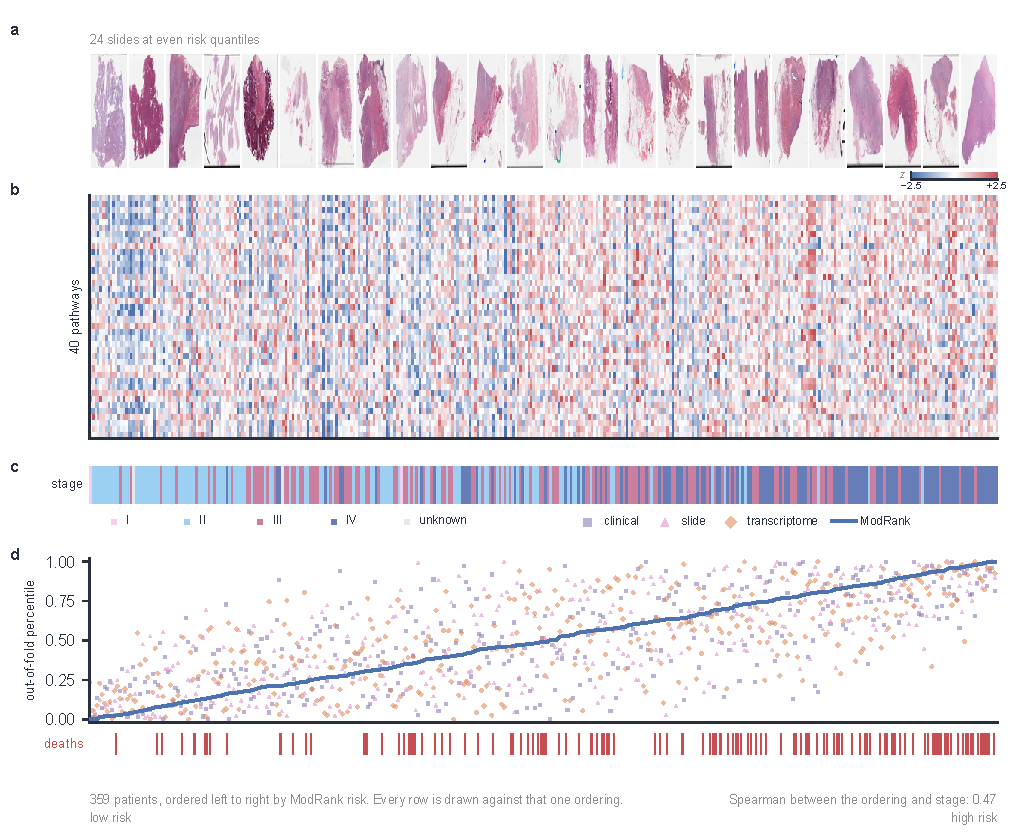
\includegraphics[width=\textwidth]{fig5_cohort_modalities.pdf}
\caption{\textbf{All three modalities across the cohort, on one patient axis.} All 359 patients,
ordered left to right by ModRank risk, with every row drawn against that one ordering.
\textbf{(a)} Twenty-four diagnostic slides sampled at even risk quantiles, at matched physical
resolution. \textbf{(b)} The forty pathways with the strongest univariate association, $z$-scored
across the cohort, one column per patient. The arm itself reads all 275. \textbf{(c)} Pathologic
stage. Higher stages are enriched to the right, as they must be, but the row is not sorted: the
Spearman correlation between the ModRank ordering and stage is 0.47, so the score is not a
re-derivation of the variable the clinical arm already carries. \textbf{(d)} The three arm
percentiles against the same ordering, with the ModRank curve drawn through them, and a rug of the
113 deaths.}
\label{fig:cohort}
\end{figure*}

\paragraph{How the clinical block was given to the comparators, and under which estimand
everything is scored.} Two details decide whether the input-parity comparison means anything, and
neither was stated. First, the clinical variables were not retrained inside either competitor. Each
competitor's own released per-case risk score is percentile-normalised within fold, the clinical
arm's percentile-normalised score is added, and the sum is re-ranked within fold. That is the
identical equal-weight rank average ModRank uses, with the competitor's joint slide-and-omics score
standing where ModRank's two molecular arms stand. We chose late fusion because retraining a
26.9-million-parameter transformer on 287 training cases to absorb six appended columns is a
different experiment with its own tuning, and because it hands the competitor the same
equal-weight rank combination that produces our own headline. It is a practical input-parity
comparator and not the only one possible. The clinical arm carries weight one half in the
competitor's average and one third in ours, and a competitor retrained with the staging variables
inside its own architecture might do better than the number we report. We have not measured
that. Second, the estimand. Our primary is a concordance pooled over all out-of-fold predictions
after within-fold percentile normalisation, whereas the convention on these folds is generally a
mean of per-fold values. On identical predictions the two differ by \textbf{+0.0034} for ModRank,
0.7239 pooled against 0.7272 as a fold mean, so the choice does not move any ranking in
Table~\ref{tab:published}. Both are reported so a reader can convert, and both reruns are scored
under whichever convention that entrant's own logged metric uses.

\subsection{What limits a method at 359 patients and 113 events}

Before designing a component we measured three things about the regime, because each has a
different correct response and they are easy to confuse.

\paragraph{The noise floor, measured on this code.} Re-splitting the same 359 cases 24 times under
an identical estimator, alpha grid, inner-CV seed and code path gives a paired between-arm delta
with SD 0.0073. Twice that, 0.0145, is the margin a claim must clear to survive a
reader re-running the study. This replaces a figure of 0.0312 the project had been carrying, which
came from a simulation at a different cohort size.

\paragraph{In-sample references on this cohort are inflated, badly.} We first estimated headroom by
fitting in-sample on the held-out fold at matched capacity and comparing against a permuted-outcome
control, and that control was the wrong one. It fitted the permutation and scored the
\emph{real} outcome, which measures whether two targets are related and answers 0.5 whatever the
capacity. Fitting the permutation and scoring \emph{that same permutation} gives the honest null:
at sixteen parameters against roughly 23 events it reaches 0.7474. The real in-sample fit
reaches 0.7666, so the excess over a matched null is $+0.0192$, and it \emph{shrinks} from $+0.0417$
at eight components as capacity grows, which is what added noise dimensions look like. The
representation was never shown to hold more than it delivers out of fold.

\paragraph{The combination rule is already at its ceiling (Fig.~\ref{fig:regime}b, c).} A 21-point weight sweep over the
image/clinical pair peaks at exactly $w=0.50$. A two-parameter fusion \emph{fitted in-sample on the
held-out fold} reaches 0.7268 against equal weighting's 0.7191, so oracle-fitted weights are
worth $+0.008$. Gating the image weight on clinical-risk tertile reaches 0.7493 against a
permuted-stratum control at 0.7502: the control wins, and by the pre-registered rule that
component is void.

Together these say that the estimator, not the fusion, is where the events are spent, and that a
method here should carry as few free parameters as the problem allows.

\begin{figure*}[t]
\centering
\includegraphics[width=\textwidth]{fig4_regime.pdf}
\caption{\textbf{What limits a method at 359 patients and 113 events.} \textbf{(a)} A ridge Cox
fitted to pure noise and scored in-sample reaches 0.7474 at sixteen parameters. The shaded band is
all a capacity increase can produce and it shrinks from $d$=8 to $d$=16. \textbf{(b)} A 21-point
weight sweep peaks at exactly equal weight. \textbf{(c)} The gated component against its
permuted-stratum control: the control wins, so the component is void by the pre-registered rule.
\textbf{(d)} Power against a true difference at this cohort's case-resampling SE. \textbf{(e)} One
competitor across five seeds. \textbf{(f)} PIBD at its best-validation checkpoint against its final
epoch, with the median published gap drawn at the same scale.}
\label{fig:regime}
\end{figure*}

\subsection{Every choice in the method answers one of those measurements}

The method is specified in Materials and methods. What belongs here is the inference from the four
measurements just reported to the four choices they force, because a design that merely happens to
be simple and a design that is simple \emph{for a reason} look identical from the outside.

\begin{itemize}
  \item One model per modality, not one joint model. A joint fit puts every coefficient
    into the same penalty and the same 113 events. Fitting each block separately spends the events
    three times over on three low-dimensional problems, and the capacity sweep is what makes that
    matter, since the excess of a real fit over its matched null \emph{shrinks} as capacity grows.
  \item A penalised linear model, not a learned head. Above sixteen parameters the
    in-sample score is dominated by what a fit to noise already achieves, so a head with more
    capacity is fitting a quantity this cohort cannot distinguish from noise.
  \item Equal weights, nothing fitted. The sweep's optimum, the oracle's margin and the
    gated component's control all say the same thing: there is no room in the combination rule, so
    we do not spend a parameter looking for it~\citep{bates1969combination}.
  \item Percentile normalisation within fold. Without it a log-hazard on one fold's scale
    is pooled against another's, and the comparison measures scale rather than skill.
\end{itemize}

\subsection{Confirmatory result}

The protocol was frozen before the run, naming the
arm, the estimator, the alpha grid, the combination rule, the comparator set, the seeds and the
decision rule. Five leakage falsifiers were executed first and two rejected: a per-fold planted
label (noise on every training row, the outcome ordering on every validation row) moved the
score by $-0.0006$, and permuting which feature row belongs to which case collapsed the arm to
$0.5127 \pm 0.0369$ over 30 draws. Seeds 1--4 had never been executed. On a benchmark with no
held-out split they are the only genuinely unseen axis, and they were put in the protocol to catch
an arm that works under one inner-CV partition only.

The primary metric (the mean pooled concordance over seeds 0--4 (Table~\ref{tab:main}, Fig.~\ref{fig:result})) is 0.7212 with SD 0.0048 across seeds, against a pre-registered target of 0.7029 and a stability bar of 0.0145. Both conditions of the rule as written are met, and the rule as written is wrong: its selection term used the standard deviation of a paired difference where the formula needs that of an absolute score, and correcting it moves the target above 0.7212. The measurement is below. Per fold the arm scores 0.6808, 0.7938,
0.7733, 0.6799 and 0.6964 (mean $0.7248 \pm 0.0545$), beating SurvPath-plus-the-same-clinical in
four of five.

Against published values on the same released folds, whose fold identity we verified where a
repository allowed it (Table~\ref{tab:published}), the arm leads the incumbent by
+0.0422. Against that incumbent's implementation given the same clinical variables (the only paired comparison the field permits, because no other entrant releases per-case predictions)
it gains +0.0340 (95\% CI $[-0.0056,\,+0.0731]$, $p=0.084$, 6{,}000 replicates resampling
\emph{cases}, never comparable pairs, since pairs sharing a patient are not independent).

\paragraph{Seed-matching the competitor, and what it costs us.} That figure is smaller than it
would be against a single run of the comparator, and the difference is instructive. SurvPath's
rerun was originally a single run at its default seed while our primary metric is a five-seed mean,
which is an asymmetry a reviewer can name. We therefore reran it at four further seeds with every
other argument unchanged. Averaged over five seeds the comparator improves from 0.6814 to
0.6897, and our margin falls from $+0.0413$ ($p=0.039$) to $+0.0340$ ($p=0.084$). We
report the seed-matched figure. Part of the apparent significance of the single-seed
comparison was the competitor having had only one noisy draw.

\paragraph{Three numbers describe ModRank and they are not interchangeable, so each is named where it is used.} The \emph{primary metric} is 0.7212, the mean of five per-seed concordances, that is the
object the pre-registered decision rule tested, and it is what Table~\ref{tab:published} reports.
Table~\ref{tab:main} is at \emph{seed 0} alone, 0.7225, because its tied-pair and within-site
columns are properties of one scoring. Every \emph{paired comparison} in this paper, including
the six-comparison family reported below and both parity comparisons, uses a
\emph{seed-averaged score vector} whose own
concordance is 0.7237, because a case-level bootstrap needs one score per patient and a mean of
concordances does not provide one. Every arm at every seed is in Supplementary Table~S4, so each
of the three can be reconstructed rather than believed. Both sides of every such comparison get the identical treatment,
and that treatment favours the competitor if it favours anyone: its seeds are full retrainings while
ours are inner-cross-validation partitions, so averaging removes more of its noise than of ours.
Reporting a single blended figure would have been simpler and would have hidden which comparison was
computed on what.

\paragraph{And the competitor's seed spread is the size of this benchmark's published gaps.}
SurvPath's concordance varies across seeds with a standard deviation of 0.0094, range
0.6112 to 0.6331, against a published 0.625 that sits near the top of that range. The nine
published entries in Table~\ref{tab:published} span 0.596 to 0.691; six of the eight gaps between
consecutive entries are 0.002 to 0.012 and the largest two are 0.021 and 0.029, for a median of
0.010. A single-run value on this benchmark is therefore a draw from a distribution that no entrant reports, and the ordering of the middle of that table is not established by the
numbers in it.

\paragraph{A second competitor at input parity, and it reveals a second unreported source of
variation.} PIBD~\citep{zhang2024pibd} is the strongest entrant besides SurvPath whose implementation
runs end to end, and its split files were byte-identical to the released ones on all five studies.
We reran it on the same folds: per fold 0.6038, 0.6980, 0.6256, 0.6147 and 0.7626, mean
$\mathbf{0.6609 \pm 0.0677}$ against a published $0.667 \pm 0.061$, a close reproduction. Its
per-case predictions were checked against ours case by case before anything was scored: 359 of 359
covered, labels, events and fold assignment identical.

PIBD writes two checkpoints per fold, one at its best \emph{validation} epoch and one at the last,
and its reported figure is a ``Best Val C-index''. The checkpoint is chosen on the very fold it is
then scored on. Both are available and both are reported here. At the best-validation
checkpoint it reaches 0.6609. At the final epoch it reaches 0.5900. The checkpoint convention
therefore moves the reported value by $+0.0709$, seven times the median gap between consecutive
entries in Table~\ref{tab:published} and more than twice the largest. That difference mixes
selection on the scored fold with the decline of a model trained to its last epoch, so it measures
what the convention is worth rather than selection optimism alone. We are not accusing anyone of misconduct: this is the
standard convention in the released code and it is how the number was always meant to be read. The
point is that a table ranking ten methods to three decimal places contains at least two effects
larger than its own resolution, seed variance and the checkpoint convention, and reports neither.

Given the same clinical variables ModRank uses, PIBD reaches 0.6989 at its best-validation
checkpoint and 0.6639 at its final epoch. Against the first (the harder comparison for us, and the one we quote) our margin is +0.0249 (95\% CI $[-0.0181,\,+0.0675]$, $p=0.241$). Against the second it is $+0.0595$ ($p=0.010$). Neither of our two input-parity margins reaches
significance under case resampling at the checkpoint convention the competitors themselves use,
and Section~\ref{sec:uncertainty} is where that is taken seriously rather than explained away.

\paragraph{What the two competitors cost, in their own trainers' words.} Both repositories print
their own parameter count at initialisation, so this is not our reconstruction of their
architectures. SurvPath's run reported a total of 24{,}702{,}532 parameters and PIBD's
26{,}930{,}702, both fully trainable. Our arm has 1{,}049: 768 slide dimensions plus
275 pathway means plus 6 clinical columns, one Cox coefficient each, and nothing fitted in
the combination at all. That is a factor of 23{,}549 and 25{,}673, on a cohort
with 113 events. We do not extend this comparison to the other eight entrants, because none of them
reports a parameter count and we did not run their code.

\begin{table*}[t]
\centering
\caption{Published values on TCGA-BLCA disease-specific survival at $n=359$, with fold identity
recorded rather than assumed. ``verified'' means the entrant's own split files were compared with
the released ones here. The upper block is on the released folds. The lower block used another
or an unverifiable protocol and is quoted as context only.}
\label{tab:published}
\begin{tabular}{llcl}
\toprule
method & venue & C-index & released folds \\
\midrule
\multicolumn{4}{l}{\emph{on the released folds, verified here or by definition}} \\
ours          & n/a                & \textbf{0.7212} & verified (definitional) \\
DIMAF~\citep{eijpe2025dimaf}          & MICCAI 2025 & 0.679 & \textbf{verified}, 5/5 folds identical \\
PIBD~\citep{zhang2024pibd}       & ICLR 2024 & 0.667 & \textbf{verified}; rerun here at $0.6609$ \\
SurvPath~\citep{jaume2024survpath} & CVPR 2024 & 0.625 & definitional \\
MOTCat~\citep{xu2023motcat}      & ICCV 2023 & 0.596 & as reported in SurvPath \\
\midrule
\multicolumn{4}{l}{\emph{another or an unverifiable protocol, quoted as context only}} \\
MOAD-FNet~\citep{moadfnet2024}   & arXiv    & 0.691 & unverified, no code released \\
APL~\citep{apl2025}              & arXiv    & 0.677 & uncheckable, repository empty \\
DSCASurv~\citep{song2025dscasurv}    & Brief.\ Bioinform.\ 2025 & 0.646 & unverified \\
OTSurv~\citep{ren2025otsurv}        & MICCAI 2025 & 0.637 & follows MMP's protocol \\
MMP~\citep{song2024mmp}          & ICML 2024 & 0.635 & own site-stratified protocol \\
\bottomrule
\end{tabular}
\end{table*}

\begin{figure*}[t]
\centering
\includegraphics[width=\textwidth]{fig3_method_result.pdf}
\caption{\textbf{The confirmatory result, and the comparisons that do not survive correction.}
\textbf{(a)} All six prespecified comparisons under Holm. Filled survives at $\alpha=0.05$, open
does not, and \textbf{both comparisons at parity in the clinical variables are among the four that do
not}. Parity here is in those variables, not in the slide encoder.
\textbf{(b)} Kaplan--Meier by risk tertile with the numbers at risk. \textbf{(c)} The incumbent as
published, beside the same predictions given the same clinical block. \textbf{(d)} IPCW
time-dependent AUC. \textbf{(e)} All seven modality subsets. \textbf{(f)} Cost against benefit. Two parameter counts are measured and the other seven entries sit on a labelled strip because no
published entry reports one.}
\label{fig:result}
\end{figure*}



\subsection{What the slide is seeing, and whether it is what the transcriptome sees}

The performance result suggests that morphology and molecules each add prognostic discrimination
to the pathology report. It says nothing about what. Eight biological axes that matter in
muscle-invasive urothelial carcinoma (Fig.~\ref{fig:biology}) were scored per case as the mean of their z-scored member
genes (basal, luminal, EMT/claudin-low, immune T-cell, proliferation, p53--cell-cycle, the FGFR3 axis, and stroma/fibroblast) with no outcome entering their construction, and the claudin genes
entered the EMT score negatively because they are \emph{lost} in that phenotype.

\paragraph{The signatures behave as this disease's literature says they should, which is the
validity check the rest of this section rests on.} Four of eight are prognostic after
Benjamini--Hochberg correction, and every one points the way it is supposed to: EMT/claudin-low
$z=+3.32$ ($q=0.007$), luminal $z=-2.81$ ($q=0.018$, protective), stroma $z=+2.71$ ($q=0.018$),
basal $z=+2.25$ ($q=0.049$). Immune T-cell infiltration points protective but does not clear
correction ($z=-1.90$, $q=0.093$), and proliferation, p53--cell-cycle and the FGFR3 axis carry no
univariate signal here.

\paragraph{The two molecular-facing arms track different biology, which is why combining them is a
decision rather than an averaging trick.} The transcriptome arm is, in effect, a molecular-subtype
reader: it correlates with luminal at $\rho=-0.372$, EMT at $+0.367$ and basal at $+0.359$, all at
$q<0.05$. The slide arm does not: its correlation with basal is $+0.044$ and does not clear
correction at all. What the slide arm tracks most strongly is the FGFR3 axis at $\rho=-0.224$, and the FGFR3 axis carries no univariate prognostic signal in this cohort ($z=-0.118$,
$q=0.906$). So the slide score is not a proxy for any of the eight standard axes. Their mutual rank
correlation is 0.271.

Over all 275 pathway scores, 59 reach $q<0.05$ against the slide arm, and the strongest are
metabolic rather than immune or subtype-related: fatty acids $\rho=-0.287$, arachidonate production
from DAG $+0.278$, ketone-body utilisation $+0.224$, glutathione synthesis and recycling $-0.219$.
These are associations between an out-of-fold model score and a pathway mean over 275 correlated
tests. They say what the score co-varies with, not that the model reads that pathway.

\paragraph{The direct test: morphology holds up where the molecules cannot separate patients.}
Restricting the comparable pairs to those the transcriptome arm separates least, the slide arm
reaches 0.6396 where the transcriptome arm itself is at 0.5604. Restricting further, to
pairs that \emph{neither} the transcriptome arm nor the clinical model can separate, each placing
the two patients within its closest 40\% (3{,}893 of 24{,}219), the slide arm still reaches 0.6212.
Morphology therefore retains prognostic discrimination among patients whom neither the
transcriptomic score nor the clinical model separates, which is the claim a
whole-slide paper has to support and the one this analysis was built to be able to refute. It
concerns these two scores and is not a proof that no transcriptomic model could recover the same
information.

\paragraph{And the two modalities are informative in different tumours.} Splitting the cohort at
the median of the basal-minus-luminal signature difference (a continuous split, since the released
files carry no subtype call), the axis is itself prognostic (log-rank $p=0.0012$) and divides the
cohort into 179 basal-leaning and 180 luminal-leaning cases. Within them (Table~\ref{tab:subtype})
the ordering of the modalities \emph{reverses}: in basal-leaning tumours the slide arm (0.6693) beats
the clinical arm (0.6472), and in luminal-leaning tumours the clinical arm (0.7005) beats the slide
arm (0.6197) by more. The combined arm sits at 0.7109 and 0.6997. It is the strongest arm in the
basal-leaning half and within 0.001 of the clinical arm in the luminal-leaning half, and it moves
far less across the split than either component that swings. That is the clearest statement of
what the combination buys: not a higher number in one place, but a number that depends less on which
molecular subtype a cohort happens to contain.

\begin{table*}[t]
\centering
\caption{Concordance within the two halves of the basal-minus-luminal signature axis, split at its
median. The slide and clinical arms swap places. The combination moves far less. The best arm in
each row is in bold.}
\label{tab:subtype}
\begin{tabular}{lccccc}
\toprule
half & $n$ / events & clinical & slide & omics & ours \\
\midrule
basal-leaning   & 179 / 71 & 0.6472 & 0.6693 & 0.6226 & \textbf{0.7109} \\
luminal-leaning & 180 / 42 & \textbf{0.7005} & 0.6197 & 0.6218 & 0.6997 \\
\bottomrule
\end{tabular}
\end{table*}

\begin{figure*}[t]
\centering
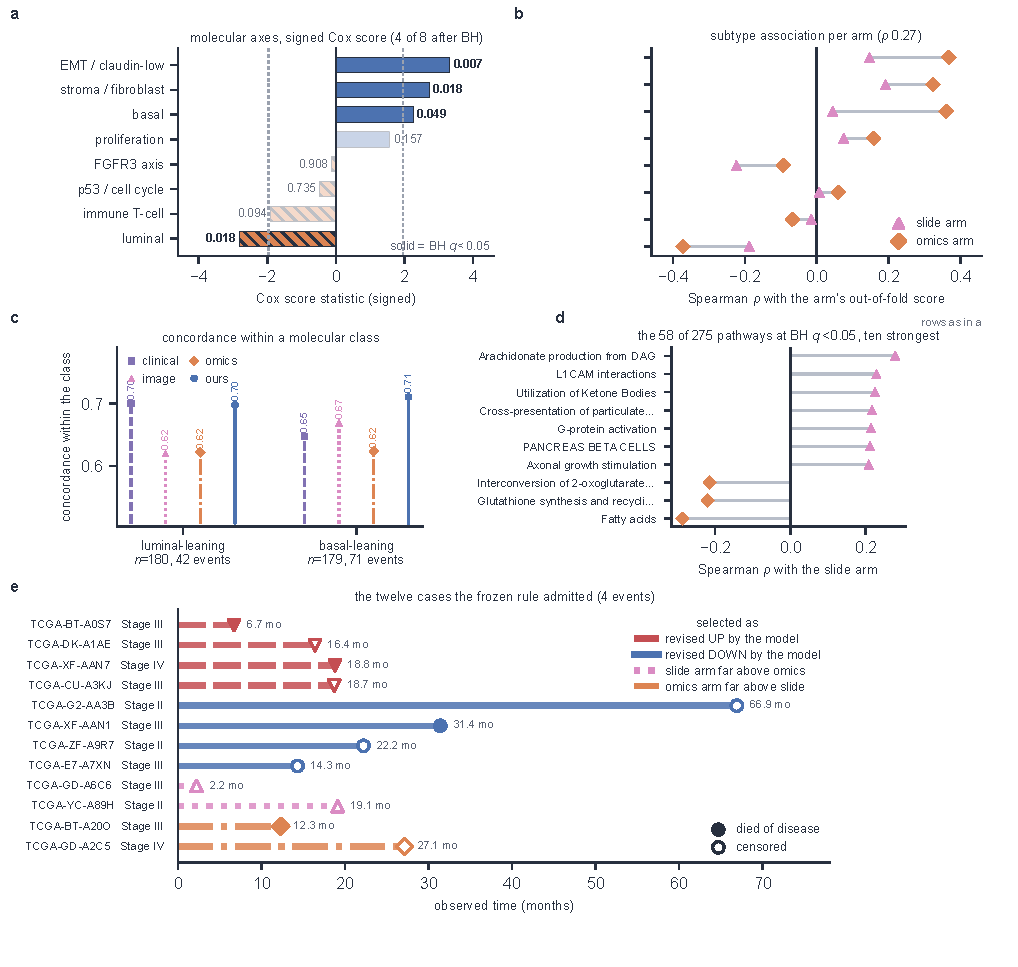
\includegraphics[width=\textwidth]{fig5_biology.pdf}
\caption{\textbf{What the two molecular-facing arms are reading.} Descriptive throughout.
\textbf{(a)} Four of eight axes are prognostic after Benjamini--Hochberg correction and each points
as this disease's literature says it should. \textbf{(b)} The omics arm is a molecular-subtype
reader. The slide arm is not. \textbf{(c)} Concordance inside a molecular class, where the class
itself carries no information. \textbf{(d)} The ten strongest of 275 pathway associations of the
slide arm. \textbf{(e)} All twelve cases the frozen rule admitted.}
\label{fig:biology}
\end{figure*}

\subsection{Two pre-registered case series, and what they actually show}

Two case series were specified before any output was inspected, and both draw from the same band, the
middle tertile of the clinical arm's out-of-fold risk (119 patients), which is where a model is
being asked to add something to the stage. They differ in what they select for, and neither replaced
the other.

The first takes the 5 highest and 5 lowest ModRank scores in that band. All ten are
reported, with their histology, in Figure~\ref{fig:cases}. The second, which Figure~\ref{fig:biology}e draws, takes the 4 highest and 4 lowest plus
the 2 largest disagreements in each direction between the slide and omics arms. Twelve cases in all, chosen to surface the modality conflicts a score ranking hides.

\begin{figure*}[t]
\centering
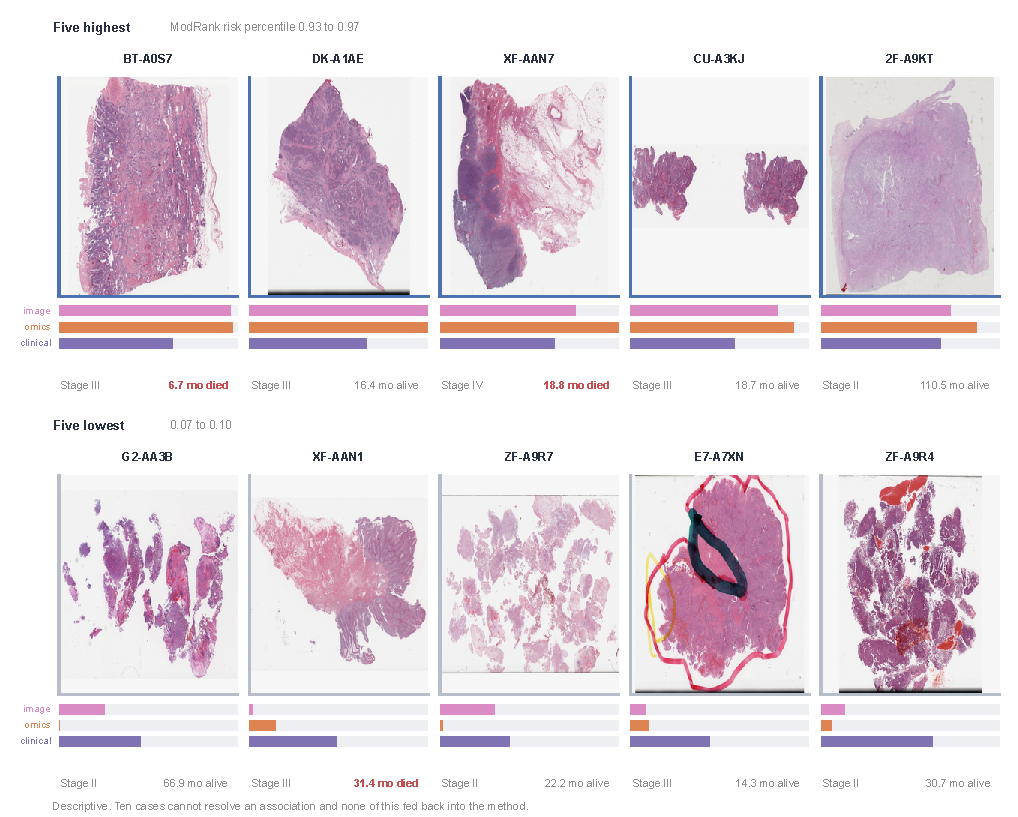
\includegraphics[width=\textwidth]{fig4_case_array.pdf}
\caption{\textbf{The ten cases the frozen rule admitted, with their histology.} The five ModRank
scores highest in the clinical middle tertile, above, and the five it scores lowest, below, with
one diagnostic slide overview per case at matched physical resolution. Under each slide the three
modality percentiles are drawn as a stack, so agreement and disagreement between morphology,
transcriptome and the report can be read per patient rather than only in aggregate. Slides are
padded rather than stretched to the cell, since distorting histology to fit a layout is not
something a figure should do. The series is reported whole, including the cases that embarrass the
model: TCGA-XF-AAN1 sits among the five lowest and died at 31.4 months, and TCGA-2F-A9KT sits among
the five highest and was alive at 110.5. Ten cases cannot resolve an association, none of this fed
back into the method, and the selection rule was fixed before any output was inspected.}
\label{fig:cases}
\end{figure*}

\paragraph{What the ten show, stated at the strength the numbers support.} The patients the method
revised \emph{upward} carry stages III, III, IV, III, II and had 2 events of five, at 6.7 and 18.8 months. Those revised
\emph{downward} carry stages II, III, II, III, II with 1 event of five, at 31.4 months. Median observed time is
18.7 months in the up-revised group against 30.7 in the down-revised. The direction is
right and the evidence is three events in ten patients, which is an illustration and not a
finding. We report it because the selection rule admitted these ten and reporting only the
agreeable ones is the failure this paper spends its Results measuring in others.

One structural feature is worth naming because it is not an outcome claim: the only stage IV patient
in either group sits among the \emph{up}-revised, and the down-revised group contains none. The
method is not simply re-deriving stage inside a band where stage was held roughly fixed.


\subsection{Where the method does not win, declared before the run}

Supplementary Figure~S1c,~d puts the two halves of the five-study evidence side by side: the method
travels to one study of five, and the defect is present in all five.

On whole-slide images and transcriptomics alone, the input set every competitor actually used, ModRank reaches 0.6841 against the incumbent's 0.679. That is $+0.0051$, inside the
noise floor, and it fails under three further combination rules and under an ensemble of seven
independently pretrained slide encoders. The lead requires the staging variables. This was
written into the frozen protocol before the run as a result declared in advance as not claimed,
and it is the reason the first result in this paper is about the benchmark's baselines rather than
about our architecture.

\subsection{Seven components, designed against measured deficits, all falsified}

Each is set out with its predicted effect, its observed effect and its matched control in
Supplementary Table~S3 and Supplementary Figure~S1a,~b.

Each carried a mechanism, a predicted slice, a falsifier fixed before the run, a removal ablation
and a matched control read \emph{before} the result (Table~\ref{tab:components}).

\begin{table*}[t]
\centering
\caption{The component slate. Bar: $+0.0145$, twice the measured split-reseed SD. \textbf{Seven
components carry an id}. Each was declared with a mechanism, a predicted slice, a falsifier, a
removal ablation and a matched control before it ran. Elastic-net Cox is listed for completeness and
has no id: it was part of the estimator slate but never reached a falsifiable comparison.}
\label{tab:components}
{\small
\begin{tabular}{cllr}
\toprule
 & component & what it did & effect \\
\midrule
C1  & pan-cancer subspace prior        & head constrained to a donor basis & $-0.0042$ \\
C1$'$ & the same direction, zero-shot    & added it to the ensemble & $+0.0033$ \\
C2  & bagged ridge                       & resampled the estimator      & $-0.056$ (image) \\
n/a & elastic-net Cox                    & changed the penalty geometry & did not converge \\
C4  & dense regularisation path          & 25 alphas, 5 inner folds     & $-0.004$ \\
C5  & gated fusion on clinical risk      & conditional combination      & \textbf{void on its control} \\
C6  & inner-CV skill weighting           & views weighted by inner-CV skill & $+0.0105$ \\
C7  & stratified partial likelihood      & within-stratum risk sets     & $-0.0199$ (tied pairs) \\
\bottomrule
\end{tabular}}
\end{table*}

One positive finding came out of the failures and is worth recording: a Cox direction fitted on
\emph{colorectal} slides, with zero case overlap, ranks \emph{bladder} patients at 0.6492 against a
permuted-label control of $0.4727 \pm 0.032$. Cross-cancer survival directions do transfer. They
simply do not improve a bladder head that already finds a better one. The cosine between the two
is 0.1748, nearly orthogonal and of comparable strength, so constraining one by the other discards
whichever is not kept.

\paragraph{What the freeze does and does not buy.} The protocol was written after the development
campaign and the leakage falsifiers had run, and before the confirmatory run. That ordering is what "frozen" means here, and the distinction matters because the word can carry more than it should. The freeze separates the run that produced the reported number from
the campaign that chose the configuration, and it fixed the arm, the estimator, the alpha grid, the
combination rule, the comparator set, the seeds and the decision rule in advance of that run. It
does not create a held-out cohort. Seeds 1 to 4 had never been executed, but a seed changes only
the inner three-fold partition that selects the penalty, so withholding them does not undo the fact
that all 269 development candidates were scored on the same 359 patients, the same outer folds and
the same representations that produce the confirmatory value. Nothing on this benchmark can undo
that, because the benchmark is a fixed cross-validation over one cohort and every published entrant
is in the same position. We therefore report the confirmatory result as what it is, a
pre-specified single execution rather than an independent validation, and the selection analysis
below is the part that carries the weight the word "confirmatory" cannot.

\paragraph{The selection correction was mis-specified, and correcting it removes the
pre-registered pass.} The decision rule set the bar at 0.679 plus a selection-inflation term
$\sigma\sqrt{2\ln N}$, pre-registered with $\sigma = 0.0073$ and $N = 211$, the number of
candidates the ledger held when the protocol was frozen, for a target of 0.7029. The campaign
finished at 269 candidates, all of them scored before the confirmatory run, and recomputing the
same term over that final count gives 0.7034, which the reported value also clears. Neither figure
is the defect. That $\sigma$ is wrong.
It is the standard deviation of a \emph{paired between-arm difference} under re-splitting, while
the expression it feeds requires the standard deviation of a candidate's own absolute score, and a
paired difference between correlated arms is smaller because common fold noise cancels. We measured
the right quantity. Permuting the time-and-event pair across cases 200 times, leaving folds,
features and estimator untouched, a single candidate's out-of-fold concordance has mean 0.5011 and
standard deviation \textbf{0.0397}, five times the figure the rule used. Substituting it gives a
bar of \textbf{0.8087}. The empirical maximum over the same candidate family, which assumes no
independence and so accounts for candidates sharing folds and components, has a 95th percentile of
0.5926, an excess over chance of 0.0926 and a bar of \textbf{0.7716}. \textbf{Under either correct
construction the primary of 0.7212 does not clear the pre-registered bar.} We report this rather
than the version that passes.

Two things qualify it and neither rescues the rule. First, a maximum-of-$N$ correction assumes the
maximum was taken, and it was not: the frozen configuration is rank \textbf{11 of the 206}
full-cohort out-of-fold candidates in the ledger, counting ties against it. Eight distinct
configurations score strictly above, two of them in a different TCGA study, three components this
paper rejects on their own pre-registered controls, and the rest the declared transcriptomic
sensitivity. The two remaining places are the frozen construction's own duplicates, recorded three
times because three sub-experiments arrived at it independently. The arm was chosen by a stated
principle and the campaign's higher-scoring configurations were discarded by it. Second, the correction is applied to
an absolute concordance against an incumbent's single published run, which the rest of this paper
argues is itself a draw from an unreported distribution. Both observations narrow what the
correction means. Neither makes 0.7212 clear a bar it does not clear, and the honest reading is
that the confirmatory decision rule was not sound enough to carry the claim it was written to
carry.

\paragraph{The lead is mostly the method and partly the encoder, and the split is measurable.}
ModRank reads a TITAN slide embedding while the comparators read their own tile features, so
``method'' and ``2025 encoder'' are confounded unless one is held fixed. We held the method fixed
and swapped the slide block through all seven encoders on identical cases and folds, with the
transcriptomic and clinical arms unchanged. The slide arm alone spans \textbf{0.1372} across
encoders, from 0.6596 for TITAN down to 0.5224 for mean-pooled UNI. The full method spans
\textbf{0.0521}, from 0.7225 to 0.6704: the combination compresses the encoder difference by a
factor of 2.6. \textbf{Five of the seven still exceed the incumbent's 0.679}, and the two that do
not are the two weakest encoders in the sweep. The two halves of this sweep sit on opposite sides of
the freeze and are labelled accordingly. All seven slide-arm values are development rows, scored
during the campaign and counted among the 269 candidates the selection term is computed over. None
of the seven full-method values is. Those were computed after the confirmatory run in response to
review, so this paragraph is a post-hoc measurement and not part of the frozen result.

None of those seven encoders is the one the comparators read, which leaves the confound answered in
general and not on the ground where it was raised. Our rerun of the weakest comparator consumed
CHIEF tile features, so we pooled those same features to the case and put them where our slide arm
goes. \textbf{The full method reaches 0.7009 on the comparator's own encoder}, above every one of
the nine published entries the benchmark carries, including the highest at 0.6910, while the
comparator that read those very features reruns at 0.6118. The CHIEF slide arm by itself is 0.5836,
below eight of the nine. The lead is therefore not an artefact of reading a better slide encoder
than the methods it is compared against. It is also not independent of the encoder: 0.7225 against
0.7009 puts that contribution near 0.022, a fifth of the margin over the incumbent and not nothing.
Both halves of that sentence are load-bearing. The reverse substitution is undefined rather than
merely expensive, because the comparators attend over a bag of four thousand patch tokens where the
public release of our slide encoder is one vector per slide.

\subsection{Three uncertainties, answering three different questions}
\label{sec:uncertainty}

\begin{itemize}
  \item Split-reseed SD 0.0073 (bar 0.0145). What moves if the same 359 patients are
    re-split. This is what a reader reproducing the study varies, and it is the right bar for a
    claim on a fixed benchmark.
  \item Selection, measured rather than assumed. Under permuted outcomes a single candidate's
    concordance has SD 0.0397, and the empirical maximum over the candidate family puts the
    bar at 0.7716, which the primary does not clear. The frozen term, computed with a paired SD
    at $N=211$, is given in Methods as what was pre-registered. This item measures how adaptive
    the development was. It is not a test the result passes.
  \item Case-level bootstrap SE $\approx 0.020$. What moves under a \emph{new} cohort of
    359. Under it NEITHER input-parity comparison reaches significance ($p=0.084$ against seed-matched SurvPath, $p=0.241$ against PIBD at its own checkpoint convention) nor does
    the comparison against the clinical arm alone. All three clear the split-reseed bar, which is
    the right instrument for a claim on a fixed benchmark. None clears the bar for a claim about a
    new cohort, and we do not make one.
\end{itemize}

At 359 patients and 113 events a concordance difference has a case-resampling SE of 0.0210, so
differences of 0.03 to 0.05 are underpowered here: 80\% power needs a true difference of 0.0589.
That is a property of this cohort, and it applies to every value in Table~\ref{tab:published},
not only to ours.

\paragraph{The whole comparison family, corrected, including the comparisons that do not survive.}
Six paired comparisons are prespecified against ModRank, and Holm's step-down procedure is applied
across all six (Fig.~\ref{fig:result}a) (Table~\ref{tab:holm}). Two survive at $\alpha=0.05$ and four do not. The
two that survive are the ones the paper's claim actually rests on, that combining the three
modalities beats either molecular modality alone. The four that do not include both comparisons at
parity in the clinical variables and the comparison against the clinical arm, which is precisely the resolution limit
described above arriving as arithmetic. The family grew from five to six when PIBD became scoreable
and Holm was recomputed over all six rather than left at the five it was first applied to. Keeping the old adjustment after adding a comparison would be the cheapest possible way to retain a result.

\begin{table*}[t]
\centering
\caption{Six prespecified comparisons against ModRank, cases resampled with 6{,}000 replicates,
Holm step-down across the whole family. Two of six survive.}
\label{tab:holm}
{\small
\begin{tabular}{lccccl}
\toprule
comparison & $\Delta$C & 95\% CI & $p$ & Holm $q$ & survives \\
\midrule
vs.\ slide alone                  & $+0.0704$ & $[+0.0288, +0.1138]$ & 0.0007 & \textbf{0.0042} & yes \\
vs.\ clinical alone               & $+0.0594$ & $[+0.0111, +0.1070]$ & 0.0163 & 0.0652 & no \\
vs.\ omics alone                  & $+0.0588$ & $[+0.0172, +0.1009]$ & 0.0053 & \textbf{0.0265} & yes \\
vs.\ ours without clinical        & $+0.0340$ & $[+0.0050, +0.0635]$ & 0.0187 & 0.0652 & no \\
vs.\ SurvPath + clinical (5 seeds) & $+0.0340$ & $[-0.0056, +0.0731]$ & 0.0843 & 0.1686 & no \\
vs.\ PIBD + clinical (best-val)   & $+0.0249$ & $[-0.0181, +0.0675]$ & 0.2413 & 0.2413 & no \\
\bottomrule
\end{tabular}}
\end{table*}

\paragraph{What margin this cohort could have detected.} At a case-resampling SE of 0.0210, 80\%
power against a two-sided $\alpha$ of 0.05 requires a true difference of 0.0589. Our
seed-matched margin over SurvPath, 0.0340, carries a power of 0.367, and our margin over PIBD,
0.0249, carries 0.220. The median gap between consecutive entries in
Table~\ref{tab:published} carries a power of 0.076, and even the largest gap in the whole table
reaches only 0.282, so the ordering of that
table's middle is not established by the numbers in it, and adding our row does not establish it
either. This is the single most useful thing we can say to the next person who runs on this
benchmark.

\paragraph{A fourth source of variation, larger than the three.} The three uncertainties above all
hold the released partition fixed. Reading concordance inside each fold separately gives a fourth
number, and it is the largest of them: ModRank spans \textbf{0.678} to \textbf{0.782} across the
five folds, a range of \textbf{0.103}, against a standard deviation of 0.0048 across seeds. The
partition itself is not balanced in events, with fold~5 carrying 16 of the 113 against 23 to 25
elsewhere. Fold-to-fold variation is therefore an order of magnitude larger than seed variation and
larger than every margin reported on this benchmark, ours included. It does not enter the primary
metric, which is defined on the released partition and must be, but a reader deciding how much of
the published ordering to believe should see it. The per-fold curves, the calibration and the
per-fold event counts are Supplementary Figure~S3.

\section{Discussion}
The result that travels furthest here is not the concordance. It is that a benchmark carrying
eleven method papers has been comparing image-and-omics models against a clinical baseline built
from tumour grade, where it compares against one at all, while pathologic stage, the variable post-operative care is built on, sat in the same
files. The consequence is quantitative, not rhetorical: on bladder the correctly specified clinical
arm reaches 0.6638, above two of the four published entries on verified folds and five of all
nine in Table~\ref{tab:published}, and within 0.016 of the incumbent. A field measuring the value added by
morphology and transcriptomics has been measuring it against the wrong reference.

Two things appear to have made this durable. The first is that the benchmark's clinical baselines were
inherited rather than re-derived (SurvPath's Supplementary Table~3 value reappears in MMP's Table~1, and DIMAF reports the same construction) so a single early choice of covariates
propagated. The second is that a clinical baseline is not a contribution any paper claims. It is the arm a method
paper runs in order to move past it, and there is no incentive anywhere in the process to make it
strong. This is the same asymmetry that makes an untuned competitor a known reviewer objection. It
is less visible when the weak arm is not a competitor's method but the clinic's own variable.

\paragraph{Comparison with previous work.} The claim that a
clinical-only reference is hard to beat is not ours. Herrmann and colleagues reached it across 18
TCGA cohorts, bladder among them, against a Cox reference built from sex, age, histological type and
tumour stage~\citep{herrmann2021benchmark}. Wissel and colleagues reached it on 17 datasets against
a clinical set that likewise carried tumour and clinical stage~\citep{wissel2023noise}. Both are
benchmarking papers about multi-omics survival models, and neither used whole-slide images.

The delta is narrow and it is the whole point. Those studies asked whether molecular blocks add over
a correctly specified clinical model and answered no. We ask a different question of a different
literature: whether the whole-slide survival family, which grew up at vision and medical-imaging
venues, inherited that clinical model at all. It did not. Where it compares against a clinical
variable it uses grade, following a lineage that runs at least from
PORPOISE~\citep{chen2022porpoise} through SurvPath~\citep{jaume2024survpath} to
MMP~\citep{song2024mmp} and DIMAF~\citep{eijpe2025dimaf}, and half of the papers examined compare against no clinical variable at all. So the finding is not that clinical baselines are
underrated, which was known. It is that one identifiable body of work has been measuring the value
of morphology against a covariate its own neighbours had already discarded, in a disease where that
covariate is near-constant, and that correcting it reorders the published table.

The second finding has no precedent we could locate. Rerunning two entrants at input parity
measured two sources of variation the benchmark's tables do not report: a competitor's spread across
seeds, and the effect of choosing a checkpoint on the fold it is then scored
on~\citep{zhang2024pibd}. Both are larger than the median gap between consecutive published entries.
We did not find a paper on this benchmark that reports either, which is a statement about our search
rather than about the field.

\paragraph{Why the method has this shape.} We are deliberately unambitious about the architecture, because the
measurements said to be. At 359 patients an in-sample fit to pure noise scores 0.7474. An
oracle-fitted fusion is worth $+0.008$. A gated fusion loses to its own permuted control. Under
those conditions the useful move is to spend the 113 events on three coefficient vectors and leave
the combination parameter-free. That the resulting method is a rank average of three penalised Cox
models, and that it leads a field of attention- and prototype-based multimodal transformers, is a
statement about the sample size rather than about deep learning. We would expect the ordering to
reverse at $n$ in the thousands, and nothing here argues otherwise.

The seven falsified components are reported for the same reason. Each was a reasonable thing to
build, several were aimed at a deficit we had measured, and all seven failed, one of them void on
its own control. A slate that is only reported when it works is a slate whose failures are
invisible to the next person, and this literature has room for the record.

\paragraph{What ``leads the benchmark'' can and cannot mean.} Our arm reports the highest
concordance yet recorded on these folds, and against the two competitors we could rerun at input
parity the margin does not reach significance under case resampling. Both statements are in this
paper, and a reader is entitled to ask which one to believe.

The answer is that they are not in tension, because the second is a property of the benchmark rather
than of the arm. The published entries do carry a fold-to-fold standard deviation (SurvPath's clinical arm is $0.570\pm0.033$, MMP's the same) but not one of them reports an interval on a
\emph{difference between methods}, or a paired test of any kind. The field ranks by point
estimates, and by that convention 0.7212 is first. A
significant paired margin is a standard \emph{no entrant here has ever met}, and this paper is
what shows why it is hard to meet at this size: 80\% power at this cohort's resampling SE requires a true
difference of 0.0589, while the median gap between consecutive published entries carries power
0.076. We therefore read the ordering of that table, ours included, as descriptive rather than
confirmatory.

So we make the weaker claim that is fully supported and decline the stronger one that is not. The
arm leads the benchmark on the benchmark's own terms. Whether leading it means what the field has
taken it to mean is the question the rest of this paper answers, and the answer is no, for every row in that table, ours included.

The lead requires the staging variables. On images and
transcriptomics alone the method is 0.6841 against an incumbent's 0.679, and no combination rule or
encoder ensemble we tried changed that. Two readings are available and we do not think the evidence
separates them: either the morphological and molecular signal genuinely adds little beyond stage at
this sample size, or the representations available to us are not the ones that would. The second is testable and was not tested here. The strongest slide encoder available, evaluated against
six alternatives, was the one we used (Supplementary Figure~S1e,~f): an arm pooling all seven is
significantly \emph{worse} than TITAN alone.

\paragraph{Limitations.}
\begin{itemize}
  \item No external validation, and none is available on this benchmark. It is
    cross-validation over 359 patients, and every published entrant is in the same position. The
    four other TCGA studies replicate the \emph{stage} finding, not the bladder number.
  \item The cohort has little power for the margins this literature reports. Under case
    resampling the SE of a concordance difference is 0.0210, so our own margin over SurvPath,
    0.0340, carries a power of 0.367. Our input-parity comparison sits at
    $p=0.084$ once the competitor is seed-matched, $p=0.241$ against the second parity
    comparator, and our comparison against the clinical arm alone at $p=0.0163$, which is
    $0.0652$ after Holm correction. All clear the split-reseed bar. None is a claim about a new
    cohort.
  \item Only two competitors could be placed at input parity, and we lead neither
    significantly. SurvPath and PIBD are the entrants whose implementations run end to end. The
    other eight rows of Table~\ref{tab:published} are quoted values that could not be given the clinical variables ModRank uses. Our margins over the two are $+0.0340$ ($p=0.084$) and
    $+0.0249$ ($p=0.241$), and neither survives Holm correction over the six-comparison family.
  \item The arm is a rank, so it carries no absolute risk by itself. Absolute risks need a hazard
    model fitted on top of it inside each training fold, and without one only the ordering is
    supported.
  \item Fold identity is unverifiable for four entrants, and three papers could not be read
    at all. We checked fold identity where a repository allowed. APL's contains two files. The
    covariate census rests on the eight papers whose text could be obtained, and the three that could not are marked as unread rather than assumed to follow the pattern.
  \item The stage finding rests on an internal comparison. Our rebuilt grade baseline does
    not reproduce the published one, most severely on COADREAD where the shipped file carries no
    usable grade. We therefore compare our grade arm against our stage arm and treat the published
    values as context.
  \item Our own clinical block was defective and was corrected mid-study, and the
    correction cost us. A cached clinical query selected the first of several diagnosis records per case. Of the 359 cases, 217 carry more than one and 61 changed. Amendment A1 did \emph{two}
    things and they pull in opposite directions: fixing the defect is worth $+0.0050$ on ModRank (95\% CI $[-0.0117,+0.0219]$, $p=0.56$), so the pre-amendment number was not inflated by the defect, while rebuilding the block from the incumbent's own four columns \emph{drops}
    the T/N/M our cached query had supplied, which is worth $-0.0110$. Net, the reported
    primary fell from 0.7260 to 0.7212, a move of $-0.0048$, the same size as the seed-to-seed SD.
    We report the lower, more conservative arm. Both values exceed the target as it was frozen,
    and neither clears it once its selection term is corrected.
\end{itemize}

\paragraph{Implications.} The immediate consequence for the benchmark is cheap to adopt: report a
clinical baseline built from the clinical covariate that discriminates in the cohort, which on this
benchmark is stage. It requires no new data, it is one column in files everyone
already downloads, and it changes what a multimodal gain means. The consequence for methods is
harder. At this cohort size the discriminating experiment between a parameter-free combination
and a learned one may not exist, and settling it needs a larger cohort rather than a better model.


\section{Conclusion}

Two results are established here and they are of different kinds. The first is a fact about a
literature: on the TCGA bladder whole-slide survival benchmark, every method paper we could read
that reports a clinical-variable baseline builds it from tumour grade, none of them uses pathologic
stage, and half the papers we could read report no clinical baseline at all. The variable was never missing from the
data. It sits in the released files, and supplying it lifts the clinical arm from 0.5666 to 0.6638
on identical cases, above two of the four published entries on verified folds and five of all
nine. The mechanism is specific and
checkable: muscle-invasive urothelial carcinoma is 94.4\% one grade level, so the covariate the
field has been comparing against cannot separate the patients it does not distinguish.

The second is a method. At 359 patients and 113 events an in-sample fit at sixteen parameters
reaches 0.7474 on pure noise, so ModRank spends its events on one penalised Cox model per modality
and none on the combination, which is an equal-weight rank average. It reaches 0.7212, the highest value reported on these folds, with 1,049 coefficients against two competitors' 25 million. It does not clear the selection-corrected bar its own decision rule should have set, and we report that alongside the number. What the same analysis also shows is that this cohort has little power for
margins of the size the literature reports, ModRank's own included, so the ranking that number wins
is a convention rather than a measurement. The correction to the baseline does not depend on that
convention, and it is the part of this paper a reader can adopt tomorrow.

\section{Competing interests}
No competing interest is declared.

\section{Author contributions statement}
G.C. conceived the study, designed and executed the analyses, and wrote the manuscript.

\section{Acknowledgments}
The author thanks the developers of SurvPath and PIBD for releasing pipelines complete enough to
be rerun end to end, and the developers of DIMAF for releasing the split files this study's
clinical block is built from. DIMAF's model was not rerun here. Two of the three findings this
paper reports about the benchmark could not have been measured without those releases.

The results published here are in whole or part based upon data generated by the TCGA Research
Network: \url{https://www.cancer.gov/tcga}. The histology shown in Figure~\ref{fig:modalities} was
read from the open-access tier of the NCI Genomic Data Commons~\citep{heath2021gdc}.

\section{Funding}
%% Supplied verbatim by the author 2026-08-17, selected from two funding sets on record. Single
%% Guangdong grant: no NSFC, no Guangdong-Hong Kong `1+1+1'. Do not copy this into another
%% manuscript -- which fund supported which work is the author's factual judgement, per paper.
This work was supported by the Guangdong Basic and Applied Basic Research Foundation
(No.~2025A1515110446).

\section{Data availability}
All data are public. The five-fold case-ID splits, the pathway definitions and the clinical columns
are those released with SurvPath (\url{https://github.com/mahmoodlab/SurvPath}). The bladder cohort
is TCGA-BLCA, with disease-specific survival from the TCGA Pan-Cancer Clinical Data Resource. No
new data were generated.

\section{Code availability}
All analysis code, the frozen benchmark protocol, the iteration ledger, the confirmatory run and the
outcome-permuted selection null are archived on Zenodo under the concept identifier
\url{https://doi.org/10.5281/zenodo.22025756}, which resolves to the most recent archived version.
Version 1.0.0, deposited on 20 August 2026 as \url{https://doi.org/10.5281/zenodo.22025757}, is the
version that produced every number reported here, and the archive carries a check script that
recomputes those numbers from the deposited result files rather than reading them from this
manuscript. The same content is held in a repository at \url{https://github.com/gxCaesar/modrank}.
Both are public.

\bibliographystyle{plain}
\bibliography{../references}

\end{document}
